\scanpage{4}
\diagram{\begin{tikzcd}[ampersand replacement=\&,column sep=1.8em,
execute at end picture={\draw[line width=.25pt] ([xshift=-2pt,yshift=-2pt]dom.south west) -- ([xshift=-2pt,yshift=-5pt]dom.south west) -- ([xshift=2pt,yshift=-5pt]gm.south east) -- ([xshift=2pt,yshift=-2pt]gm.south east);}]
N\unsure{\mathpunct{;}|\mathpunct{:}}\& |[alias=dom]| S_E \arrow[r] \& S_{\mathbb{Q}}\arrow[r] \& |[alias=gm]| {\mathbb{G}_{m}}
\end{tikzcd}}

\[
(x,(y_{\alpha}))\longrightarrow x\cdot
\prod_{\alpha<\infty}\lVert y_{\alpha}\rVert\cdot
\prod_{\alpha=\infty}\operatorname{sign}(y_{\alpha})
\]

\margin{$\unsure{\ell|1}$}
\diagram{\begin{tikzcd}[ampersand replacement=\&,column sep=2.1em]
|[alias=csource]| C(E)\arrow[r]\arrow[rr,bend right=24,swap,"{\text{\uuline{$\lVert x\rVert$}}}"] \&
S_E\inserted{(\mathbb{A})}\arrow[r] \&
\unsure{S|\deleted{S}}_{\unsure{E|\epsilon}}(R)\arrow[r] \& \mathbb{R}^{*}
\end{tikzcd}}

\figure{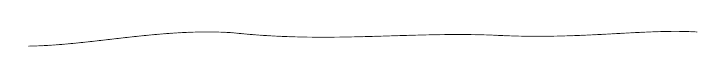
\begin{tikzpicture}[x=1cm,y=1cm]
\draw[line width=.25pt] (0,0) .. controls (.8,.01) and (1.7,.23) .. (2.6,.17) .. controls (3.8,.04) and (4.8,.18) .. (5.9,.14) .. controls (7,.08) and (7.8,.22) .. (8.5,.18);
\end{tikzpicture}}
\figure{\begingroup
\setbox0=\hbox{$-1\ne\lVert-1\rVert\unsure{\mathpunct{.}|\mathpunct{:}}$}
\leavevmode\rlap{\begin{tikzpicture}[baseline=0pt]
\coordinate (sw) at (-3pt,-3pt);
\coordinate (nw) at (-3pt,\dimexpr\ht0+3pt\relax);
\coordinate (ne) at (\dimexpr\wd0+3pt\relax,\dimexpr\ht0+3pt\relax);
\coordinate (se) at (\dimexpr\wd0+3pt\relax,-3pt);
\draw[line width=.25pt] ([xshift=-1pt]sw) .. controls ([xshift=-3pt]nw) and (nw) .. ([xshift=6pt,yshift=1pt]nw);
\draw[line width=.25pt] ([xshift=6pt]nw) .. controls (nw) and (ne) .. ([xshift=2pt,yshift=-3pt]ne) -- (se);
\end{tikzpicture}}\box0\endgroup}
% archive sheet number: 3
\clearpage
